\section{Results}

\subsection{Reference cases reproduce the intended passive ordering}

The baseline reference configuration generated the intended progression from near-isopotential head-dendrite responses to strong local isolation (Figures~\ref{fig:architecture} and \ref{fig:baseline_validation}). The simulations used the baseline parameters in Table~\ref{tab:parameters}, $\Delta t=0.01$ ms, a single head synapse at 20 ms, and the predefined 50 ms metric window. All nine low-, intermediate-, and high-isolation target values passed the predefined tolerance rule.

The low-SMI case produced $\SMI=0.00881$, $\Ghd=0.984$, $\Ghs=0.357$, and $\Ah=1.82$ mV. The intermediate case produced $\SMI=0.115$, $\Ghd=0.751$, $\Ghs=0.273$, and $\Ah=2.36$ mV. The high-SMI case produced $\SMI=1.32$, $\Ghd=0.102$, $\Ghs=0.0376$, and $\Ah=15.1$ mV. These target cases support implementation consistency for the reference equations, units, synaptic normalization, solver, and metric definitions in the compact passive architecture; they do not calibrate the model to a specific biological neuron.

The same traces show why the divider residual is needed. The baseline divider predictions were 0.991, 0.897, and 0.431 for the low, intermediate, and high cases. The corresponding residuals $\Ghd-\Gamma_{\mathrm{div}}$ were -0.00729, -0.1458, and -0.3286. The low case was close to the DC divider, whereas the intermediate and high transient peak ratios fell well below it.

\begin{figure}[!htbp]
\centering
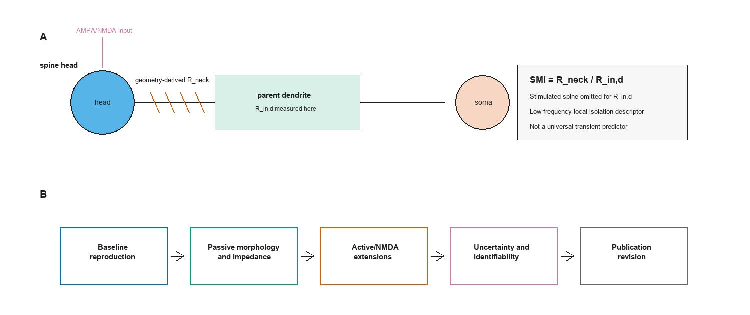
\includegraphics[width=\textwidth,height=0.34\textheight,keepaspectratio]{figures_publication/Fig1_architecture.pdf}
\caption{\textbf{SPINE reference architecture and residual workflow.} A conductance-based excitatory input drives an explicit spine head coupled to the parent dendrite through a geometry-derived neck resistance. The dendrite-soma input resistance is measured after omitting the stimulated spine, yielding $\SMI=\Rneck/\Rin$ and the analytic local divider expectation $\Gamma_{\mathrm{div}}=1/(1+\SMI)$.}
\label{fig:architecture}
\end{figure}

\begin{figure}[!htbp]
\centering
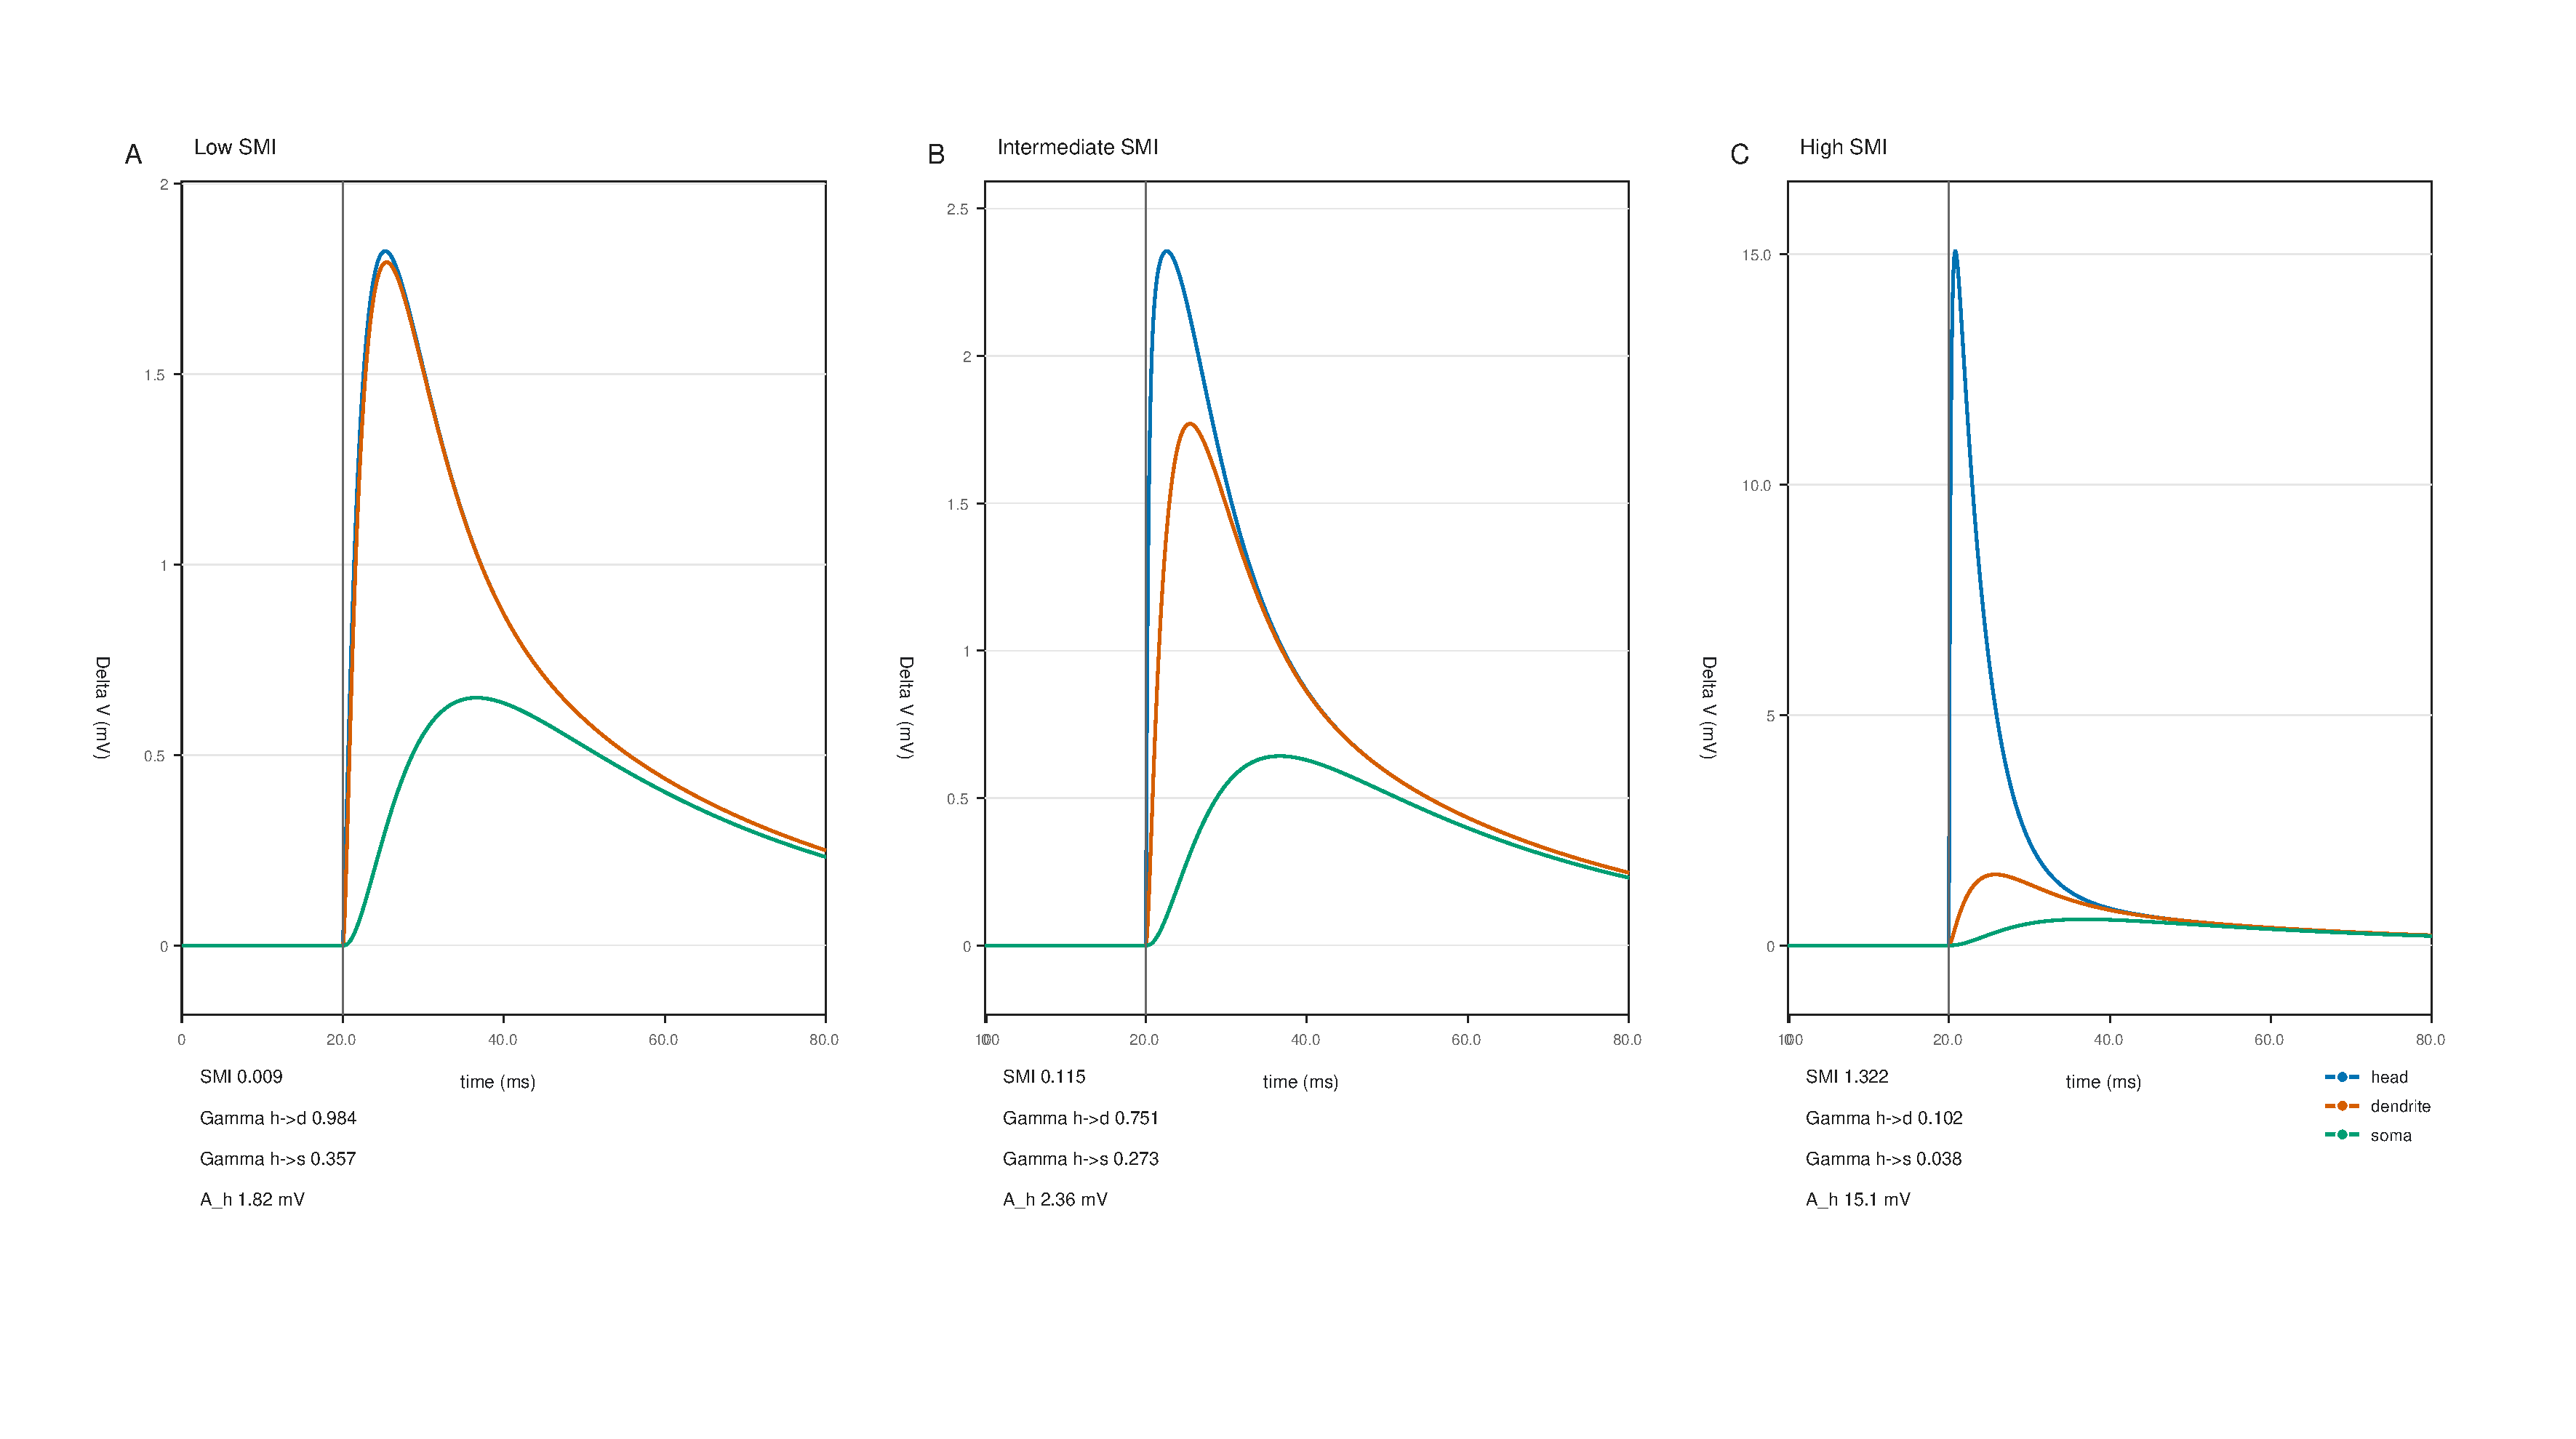
\includegraphics[width=\textwidth,keepaspectratio]{figures_publication/Fig2_baseline_traces.pdf}
\caption{\textbf{Baseline passive reference traces.} Low-, intermediate-, and high-SMI traces show the intended local coupling progression. The reference cases also demonstrate that target-case ordering does not imply exact equality to the DC divider: residuals are small for the low case and larger for intermediate/high transient peak responses.}
\label{fig:baseline_validation}
\end{figure}

\subsection{The analytic divider is a reference, not the peak-response result}

Across 3718 existing residual rows, the median absolute residual from the divider was 0.0548, the mean absolute residual was 0.0734, and the root-mean-square residual was 0.103. The maximum absolute residual was 0.492. Residuals were negative in 3680 rows and positive in 38 rows, so the DC divider usually overpredicted the observed conductance-based peak local transfer (Figure~\ref{fig:divider_residuals}).

The largest departures were scientifically informative rather than numerical defects. The matched-neck heterogeneous-load sweep produced the largest absolute residual, with $\SMI=0.452$, observed $\Ghd=0.196$, divider prediction 0.689, and residual -0.492. Fixed-load high-SMI rows also showed large relative departures. These patterns are consistent with the distinction between a low-frequency small-signal divider and a transient conductance-driven peak voltage ratio.

Excluding exploratory rows left the same conclusion: 3584 non-exploratory rows had median absolute residual 0.0563, mean absolute residual 0.0748, and only two positive residual rows. The divider relation therefore remains the correct analytic baseline, but the residual field is the empirical domain-of-validity map.

\begin{figure}[!htbp]
\centering
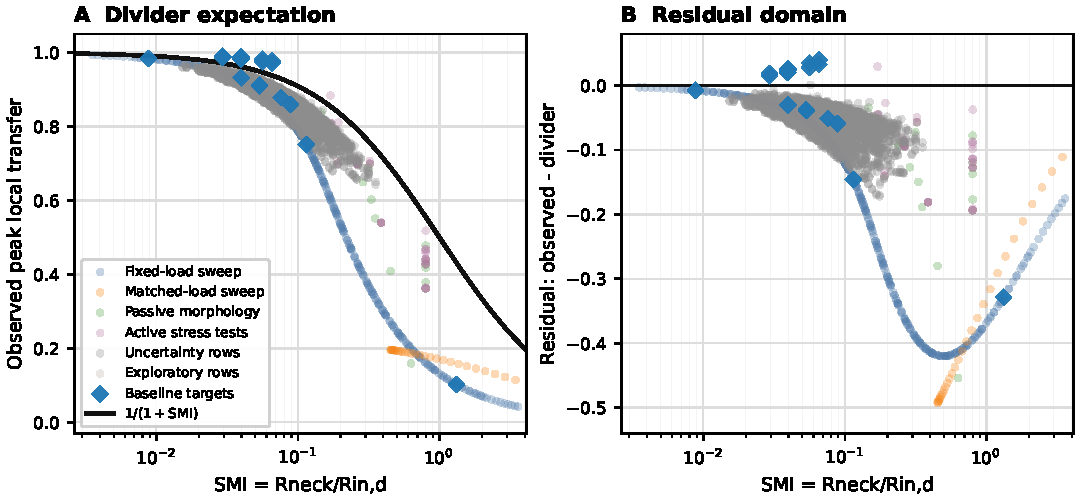
\includegraphics[width=\textwidth,keepaspectratio]{figures_publication/Fig3_divider_residuals.pdf}
\caption{\textbf{Analytic divider overlay and residual domain.} Observed peak local transfer is compared with the DC divider expectation $\Gamma_{\mathrm{div}}=1/(1+\SMI)$ across 3718 derived rows. Most points fall below the divider curve, and the residual panel makes the departure visible. Baseline targets are highlighted; exploratory rows are included only as separated stress-test context.}
\label{fig:divider_residuals}
\end{figure}

\subsection{Load normalization is useful but compact}

The fixed-load geometry sweep behaved as a constructional sanity check. Longer and narrower necks increased $\Rneck$, increased head depolarization, and decreased downstream transfer. Because $\Rin$ was fixed, $\SMI$ and $\Rneck$ had identical rank ordering. This result should not be read as evidence that the ratio adds information under fixed-load conditions.

The matched-neck experiment held $\Rneck=100$ M$\Omega$ while varying dendritic leak from 0.1 to 30 nS (Figure~\ref{fig:fixedload}). Under this manipulation, neck resistance alone could not rank the cases because there was only one neck-resistance value. Changing the dendritic load changed $\Rin$, and therefore changed $\SMI$ and downstream transfer. The load term is therefore mechanistically meaningful, but only within the target it was designed to represent.

Phase 2 descriptor comparisons made this compactness explicit. For non-exploratory local transfer, $\SMI$ and $\Gamma_{\mathrm{div}}$ had the same absolute Spearman association because the divider is a monotone transform of the ratio, but the analytic divider was the better direct scalar prediction (cross-validated RMSE 0.052 versus 0.091 for raw $\SMI$). The log component pair improved on raw $\SMI$ but did not outperform the analytic divider for first-order local transfer. Thus the ratio is useful as the coordinate defining the divider, not as a universally superior scalar.

\begin{figure}[!htbp]
\centering
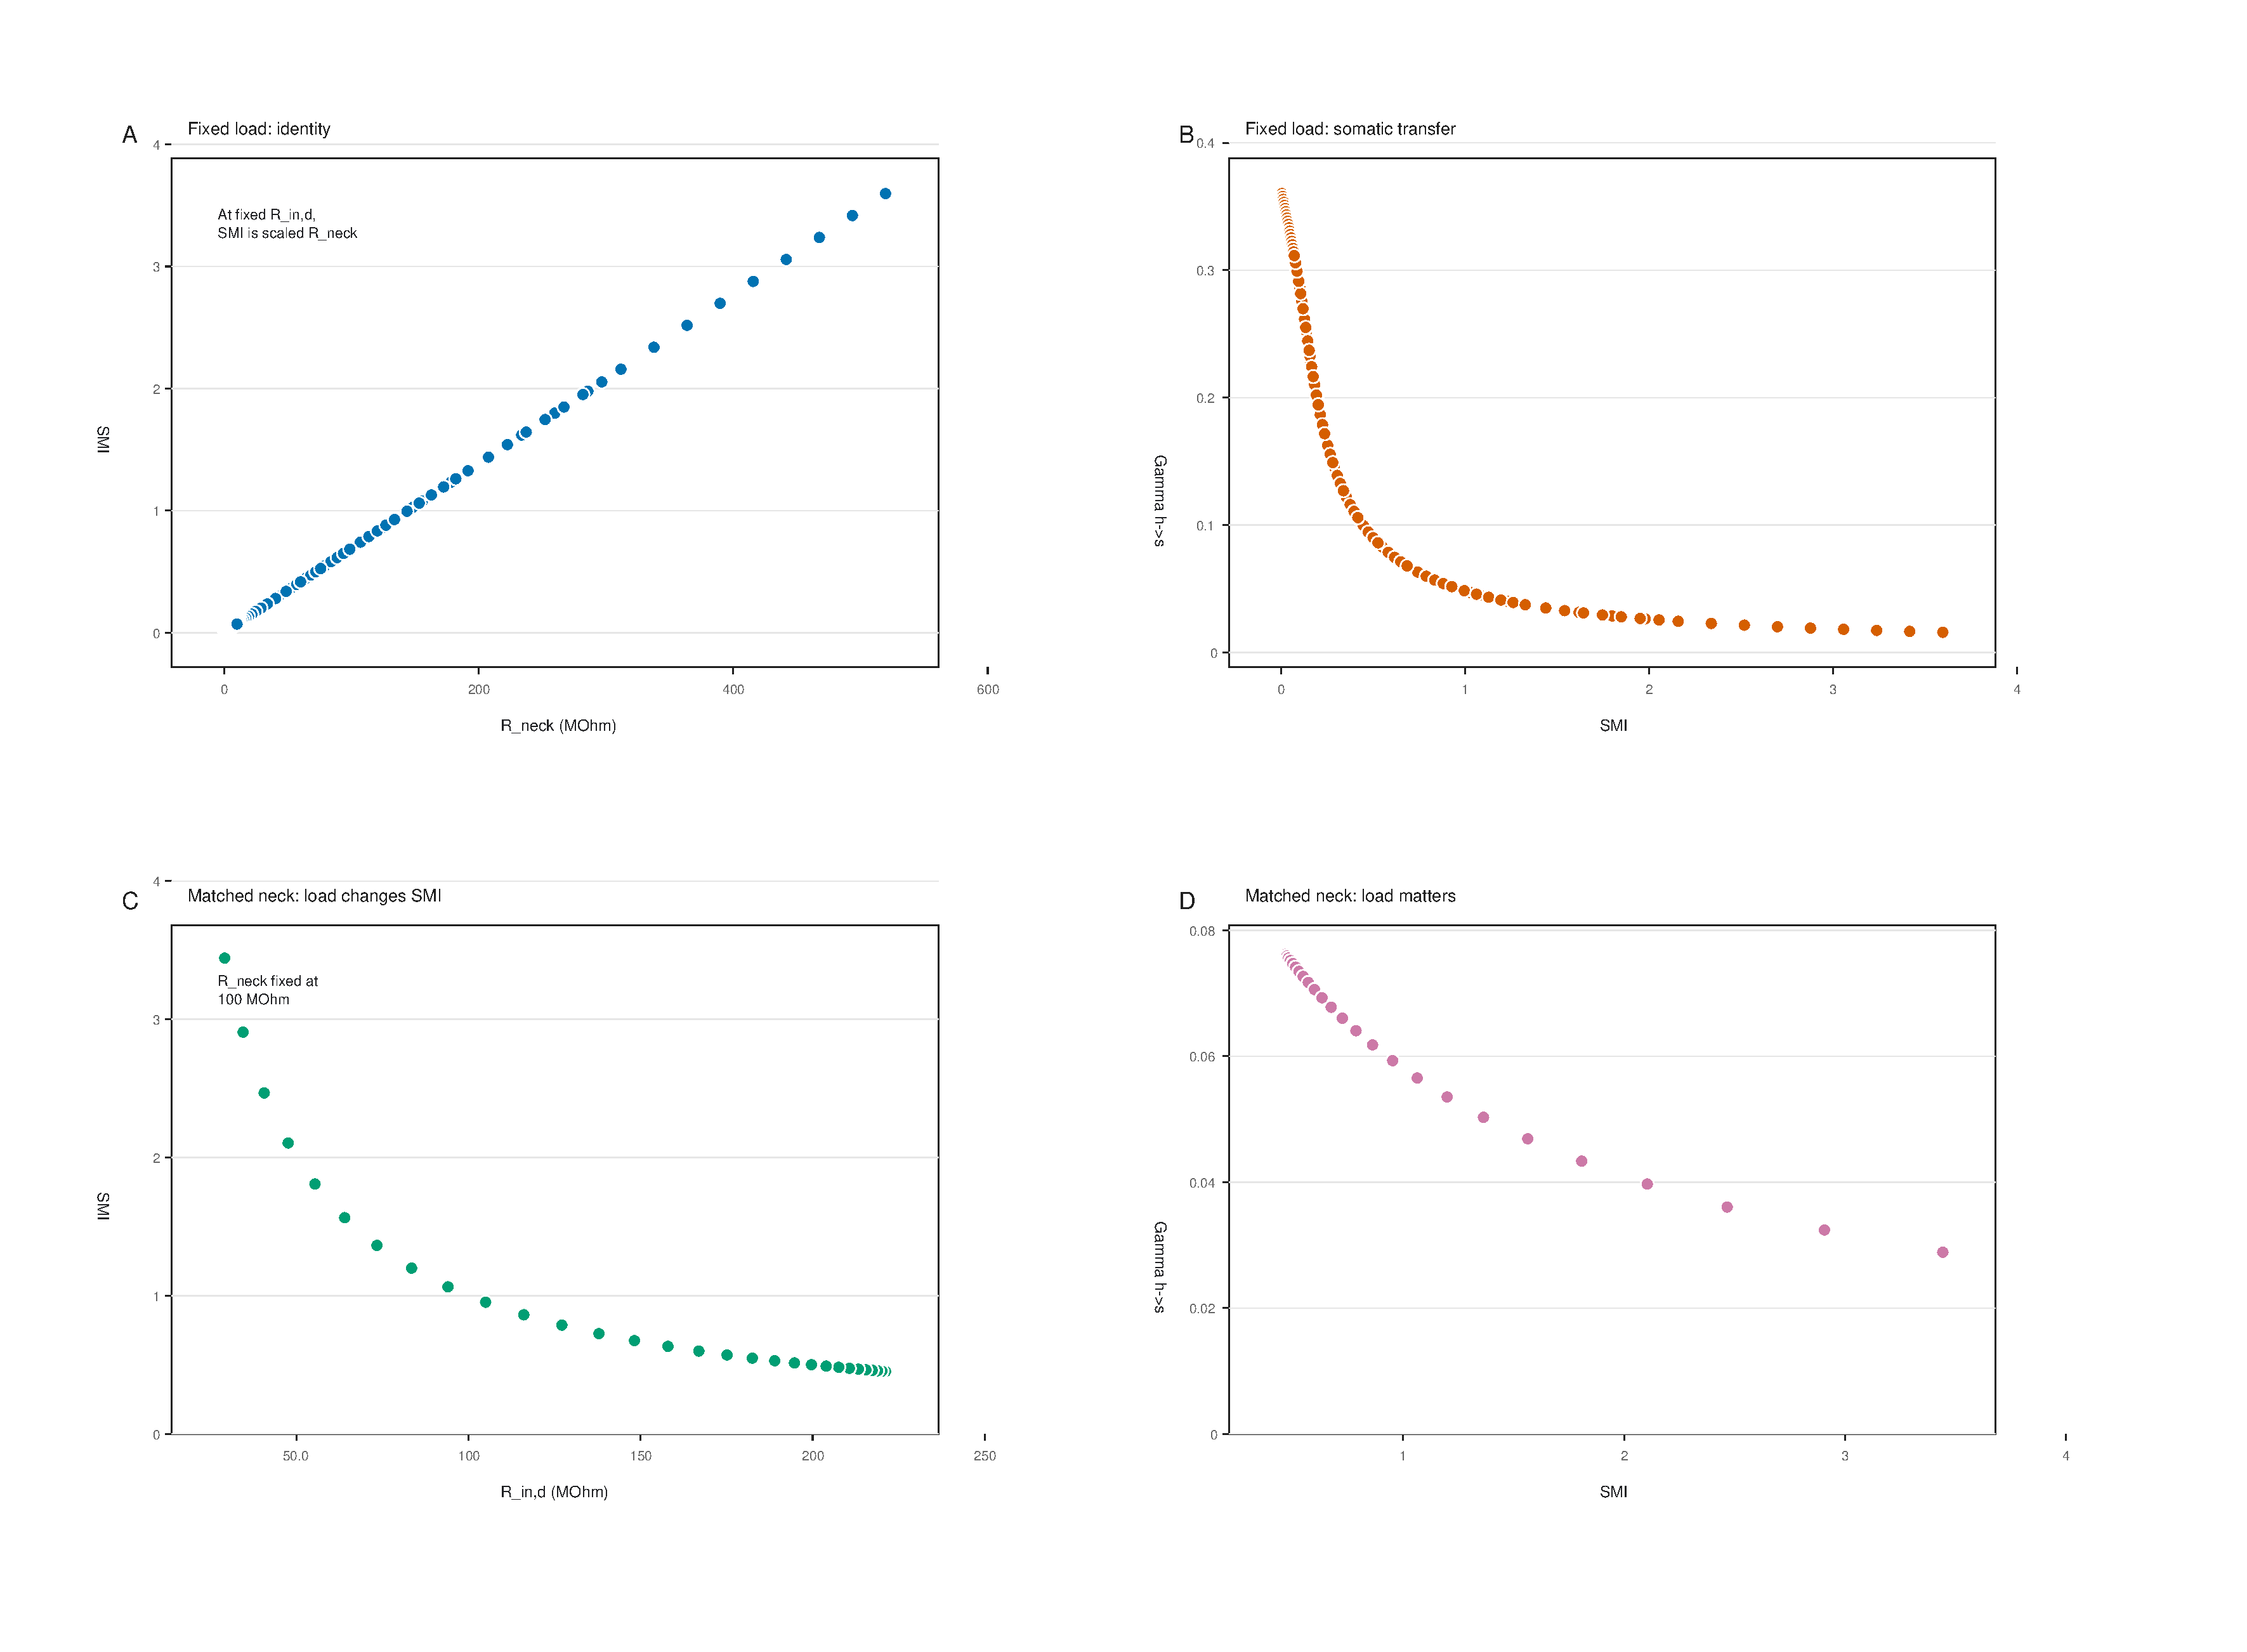
\includegraphics[width=\textwidth,keepaspectratio]{figures_publication/Fig3_load_normalization.pdf}
\caption{\textbf{Fixed-load and matched-neck controls.} At fixed dendritic input resistance, $\SMI$ is a scaled neck-resistance coordinate. When $\Rneck$ is held fixed and dendritic load changes, the ratio changes with $\Rin$ and separates cases that neck resistance alone cannot order.}
\label{fig:fixedload}
\end{figure}

\subsection{Residuals, amplitude, and somatic transfer require richer descriptors}

The residual analysis separated local-divider usefulness from broader prediction. For signed and absolute divider residuals, dynamic SMI was the strongest available scalar by rank association (absolute Spearman 0.853), while $\Rneck$ exceeded raw $\SMI$ (about 0.765 versus 0.704). In rows with synaptic conductance scale, conductance plus log-component models sharply reduced residual prediction error. Residuals are therefore better treated as a dynamic/conductance/impedance problem than as evidence that the DC ratio alone is sufficient.

Head amplitude was still more target-specific. Across non-exploratory rows, synaptic conductance scale had absolute Spearman association 0.982 with $\Ah$, whereas raw $\SMI$ was only 0.143. Somatic transfer depended on downstream filtering: transfer gain and transfer impedance exceeded raw $\SMI$ for $\Ghs$ in the Phase 2 summary. These results support a target-specific descriptor interpretation: local divider reasoning, head amplitude, residuals, and somatic transfer require different descriptor families.

Designed passive counterexamples sharpened this interpretation. Passive iso-SMI cases with different morphology produced relative spread 0.28 in $\Ghd$ and 0.61 in $\Ah$, both exceeding the predefined 20\% failure threshold. Equal $\SMI$ is therefore not electrical equivalence, because the same ratio can hide different absolute resistances, capacitances, impedance spectra, synaptic drives, and downstream morphologies.

\begin{figure}[!htbp]
\centering
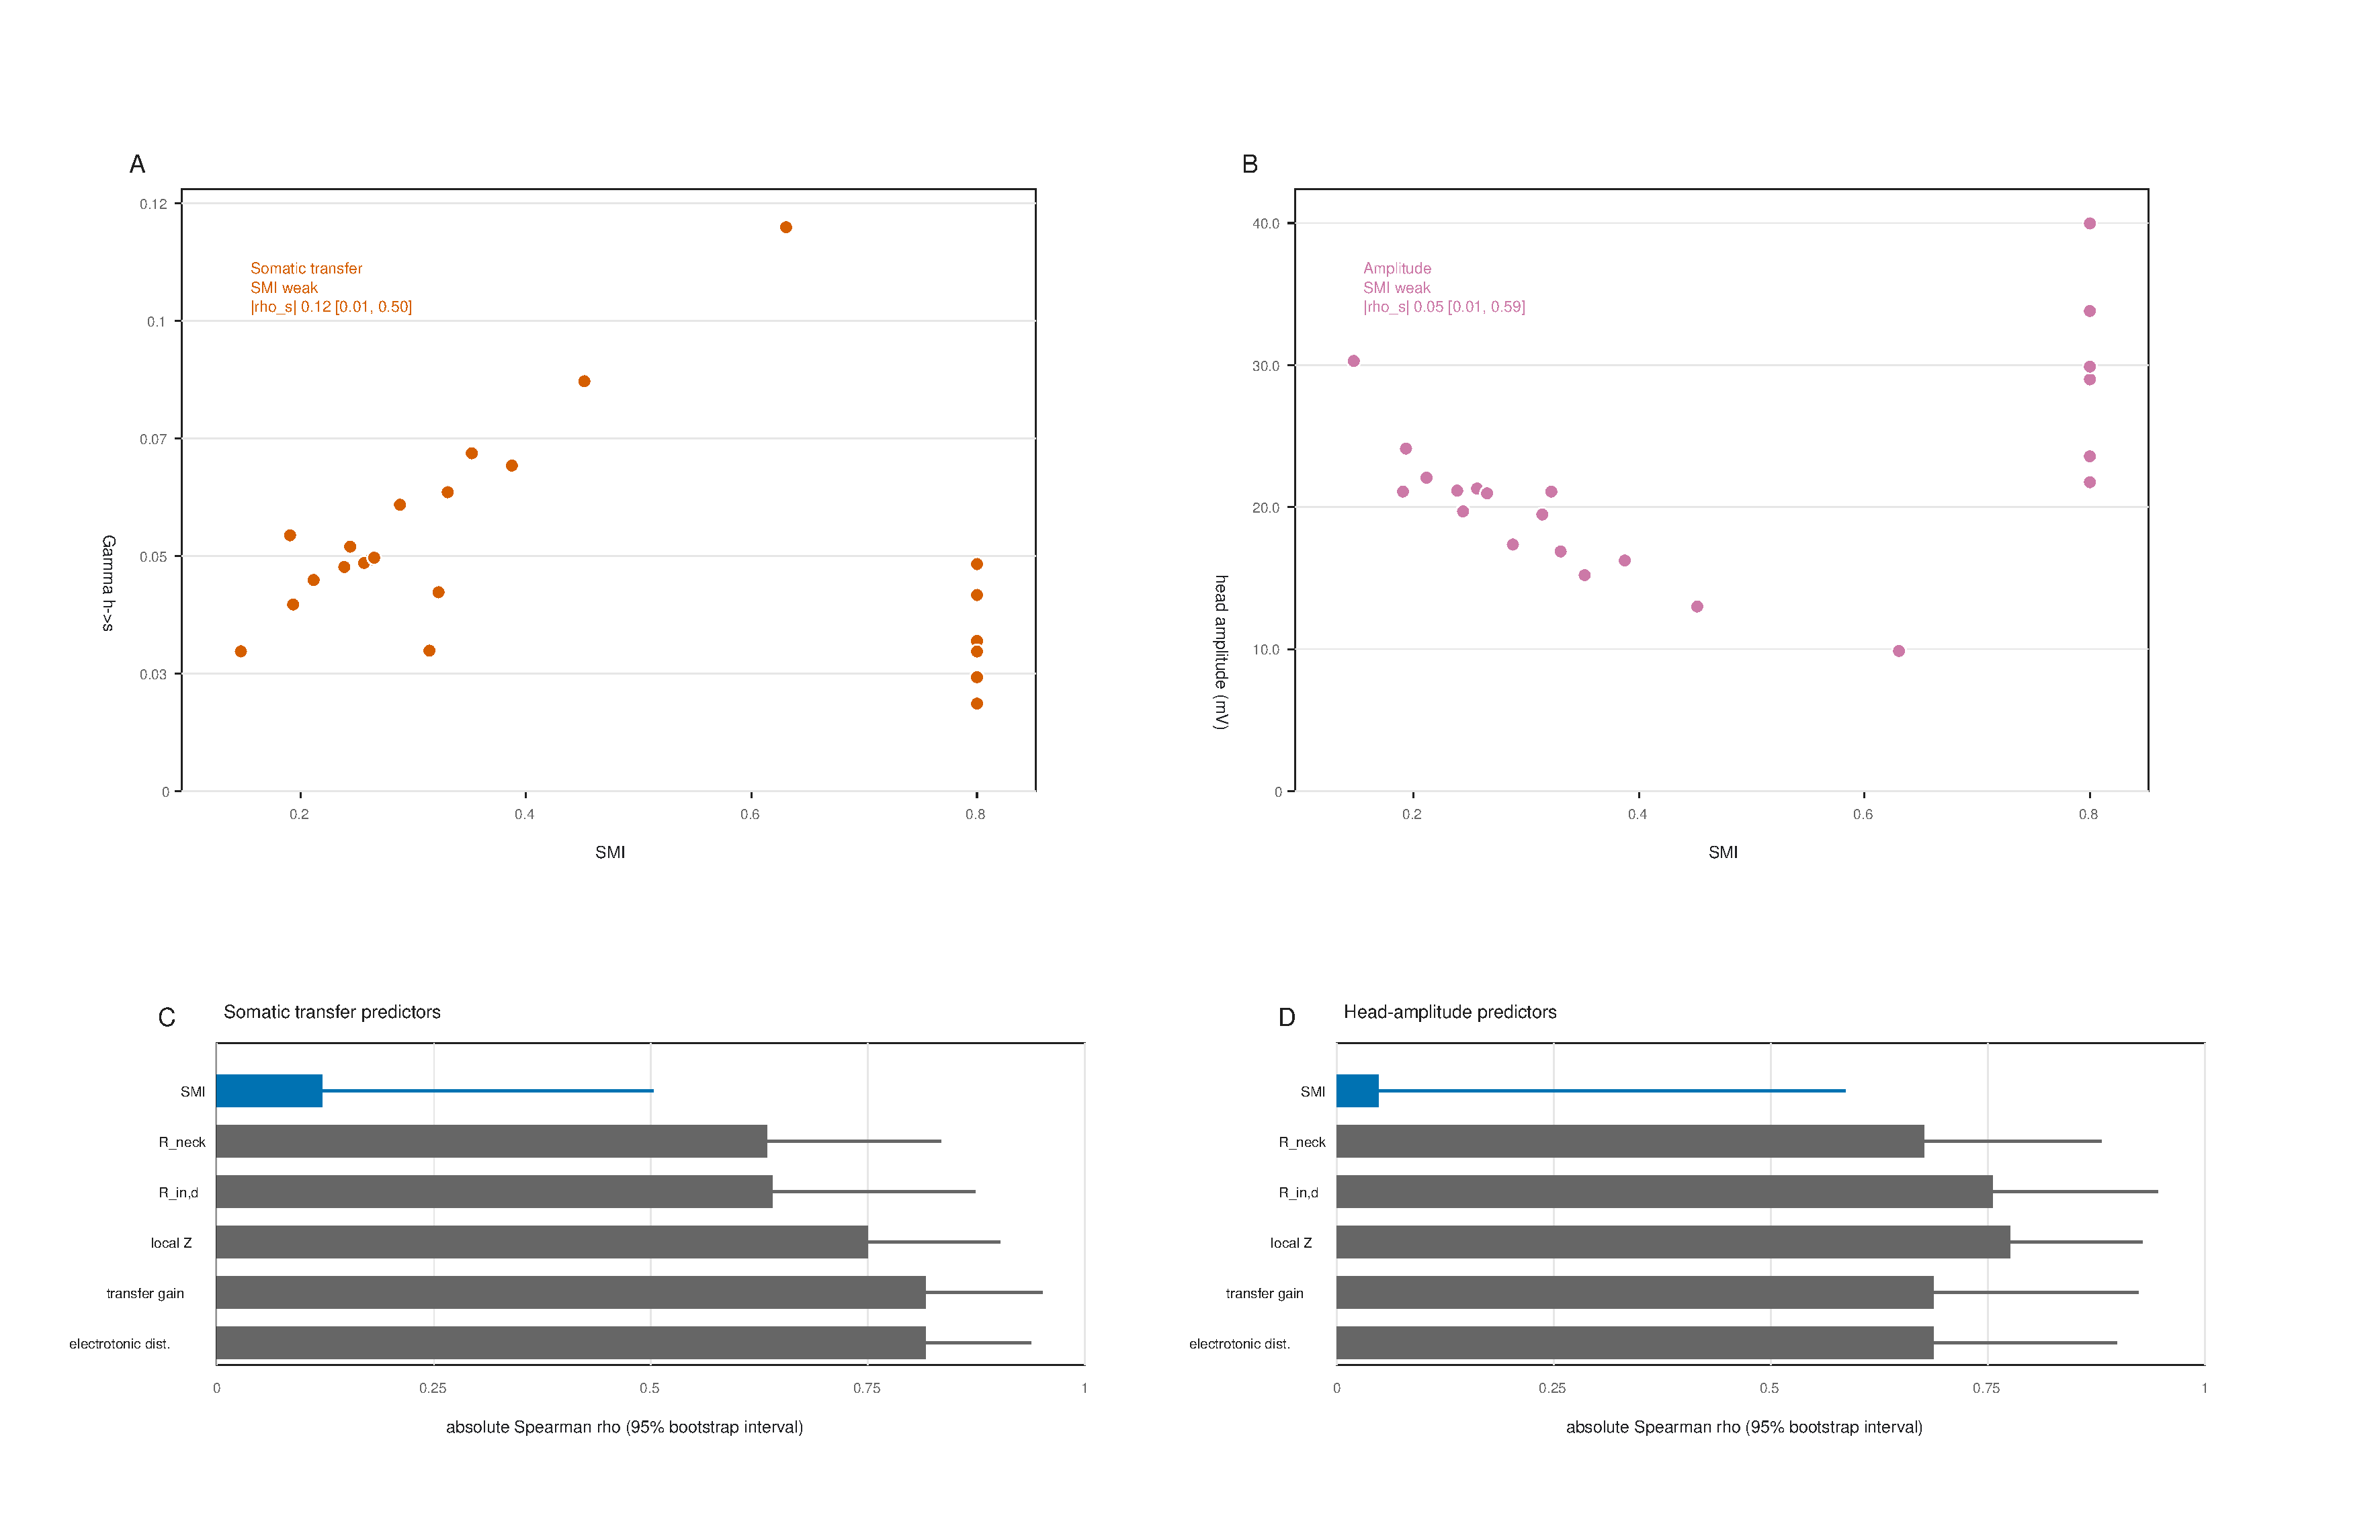
\includegraphics[width=\textwidth,keepaspectratio]{figures_publication/Fig5_passive_limitations.pdf}
\caption{\textbf{Passive limits of the compact ratio.} Passive challenge rows show that local-divider information does not automatically transfer to head amplitude or somatic voltage. Component, impedance, transfer-gain, and synaptic-drive descriptors retain information that the ratio discards.}
\label{fig:passivefailures}
\end{figure}

\subsection{Active and NMDA stress tests preserve scope limits}

Active validation passed all 12 predefined rows, including AMPA peak normalization, NMDA magnesium-block monotonicity, NMDA current-voltage relief, active-current signs, bounded gates, resting-state stability, timestep refinement, limiting-case solver comparison, strong-drive stability, and unit conversion checks. Active mechanisms were disabled in the reference baseline and enabled only in active-extension protocols.

In the designed active nonlinear suite, $\SMI$ remained strongly associated with local $\Ghd$, but active mechanisms did not make the static ratio a general amplitude or somatic-transfer predictor (Figure~\ref{fig:active}). For active $\Ghs$, input impedance at 50 Hz exceeded raw $\SMI$ (0.764 versus 0.339). For active $\Ah$, frozen-gate transfer gain exceeded raw $\SMI$ (0.736 versus 0.236). AMPA+NMDA protocols with full restrained active conductances produced iso-SMI relative spread 0.86 in $\Ah$ and 0.35 in $\Ghd$, exceeding the predefined active stress-test thresholds.

Thus active mechanisms do not overturn the divider framing; they make its scope more important. Voltage-dependent current and active state add response variables that are not contained in a static morphology/load ratio.

\begin{figure}[!htbp]
\centering
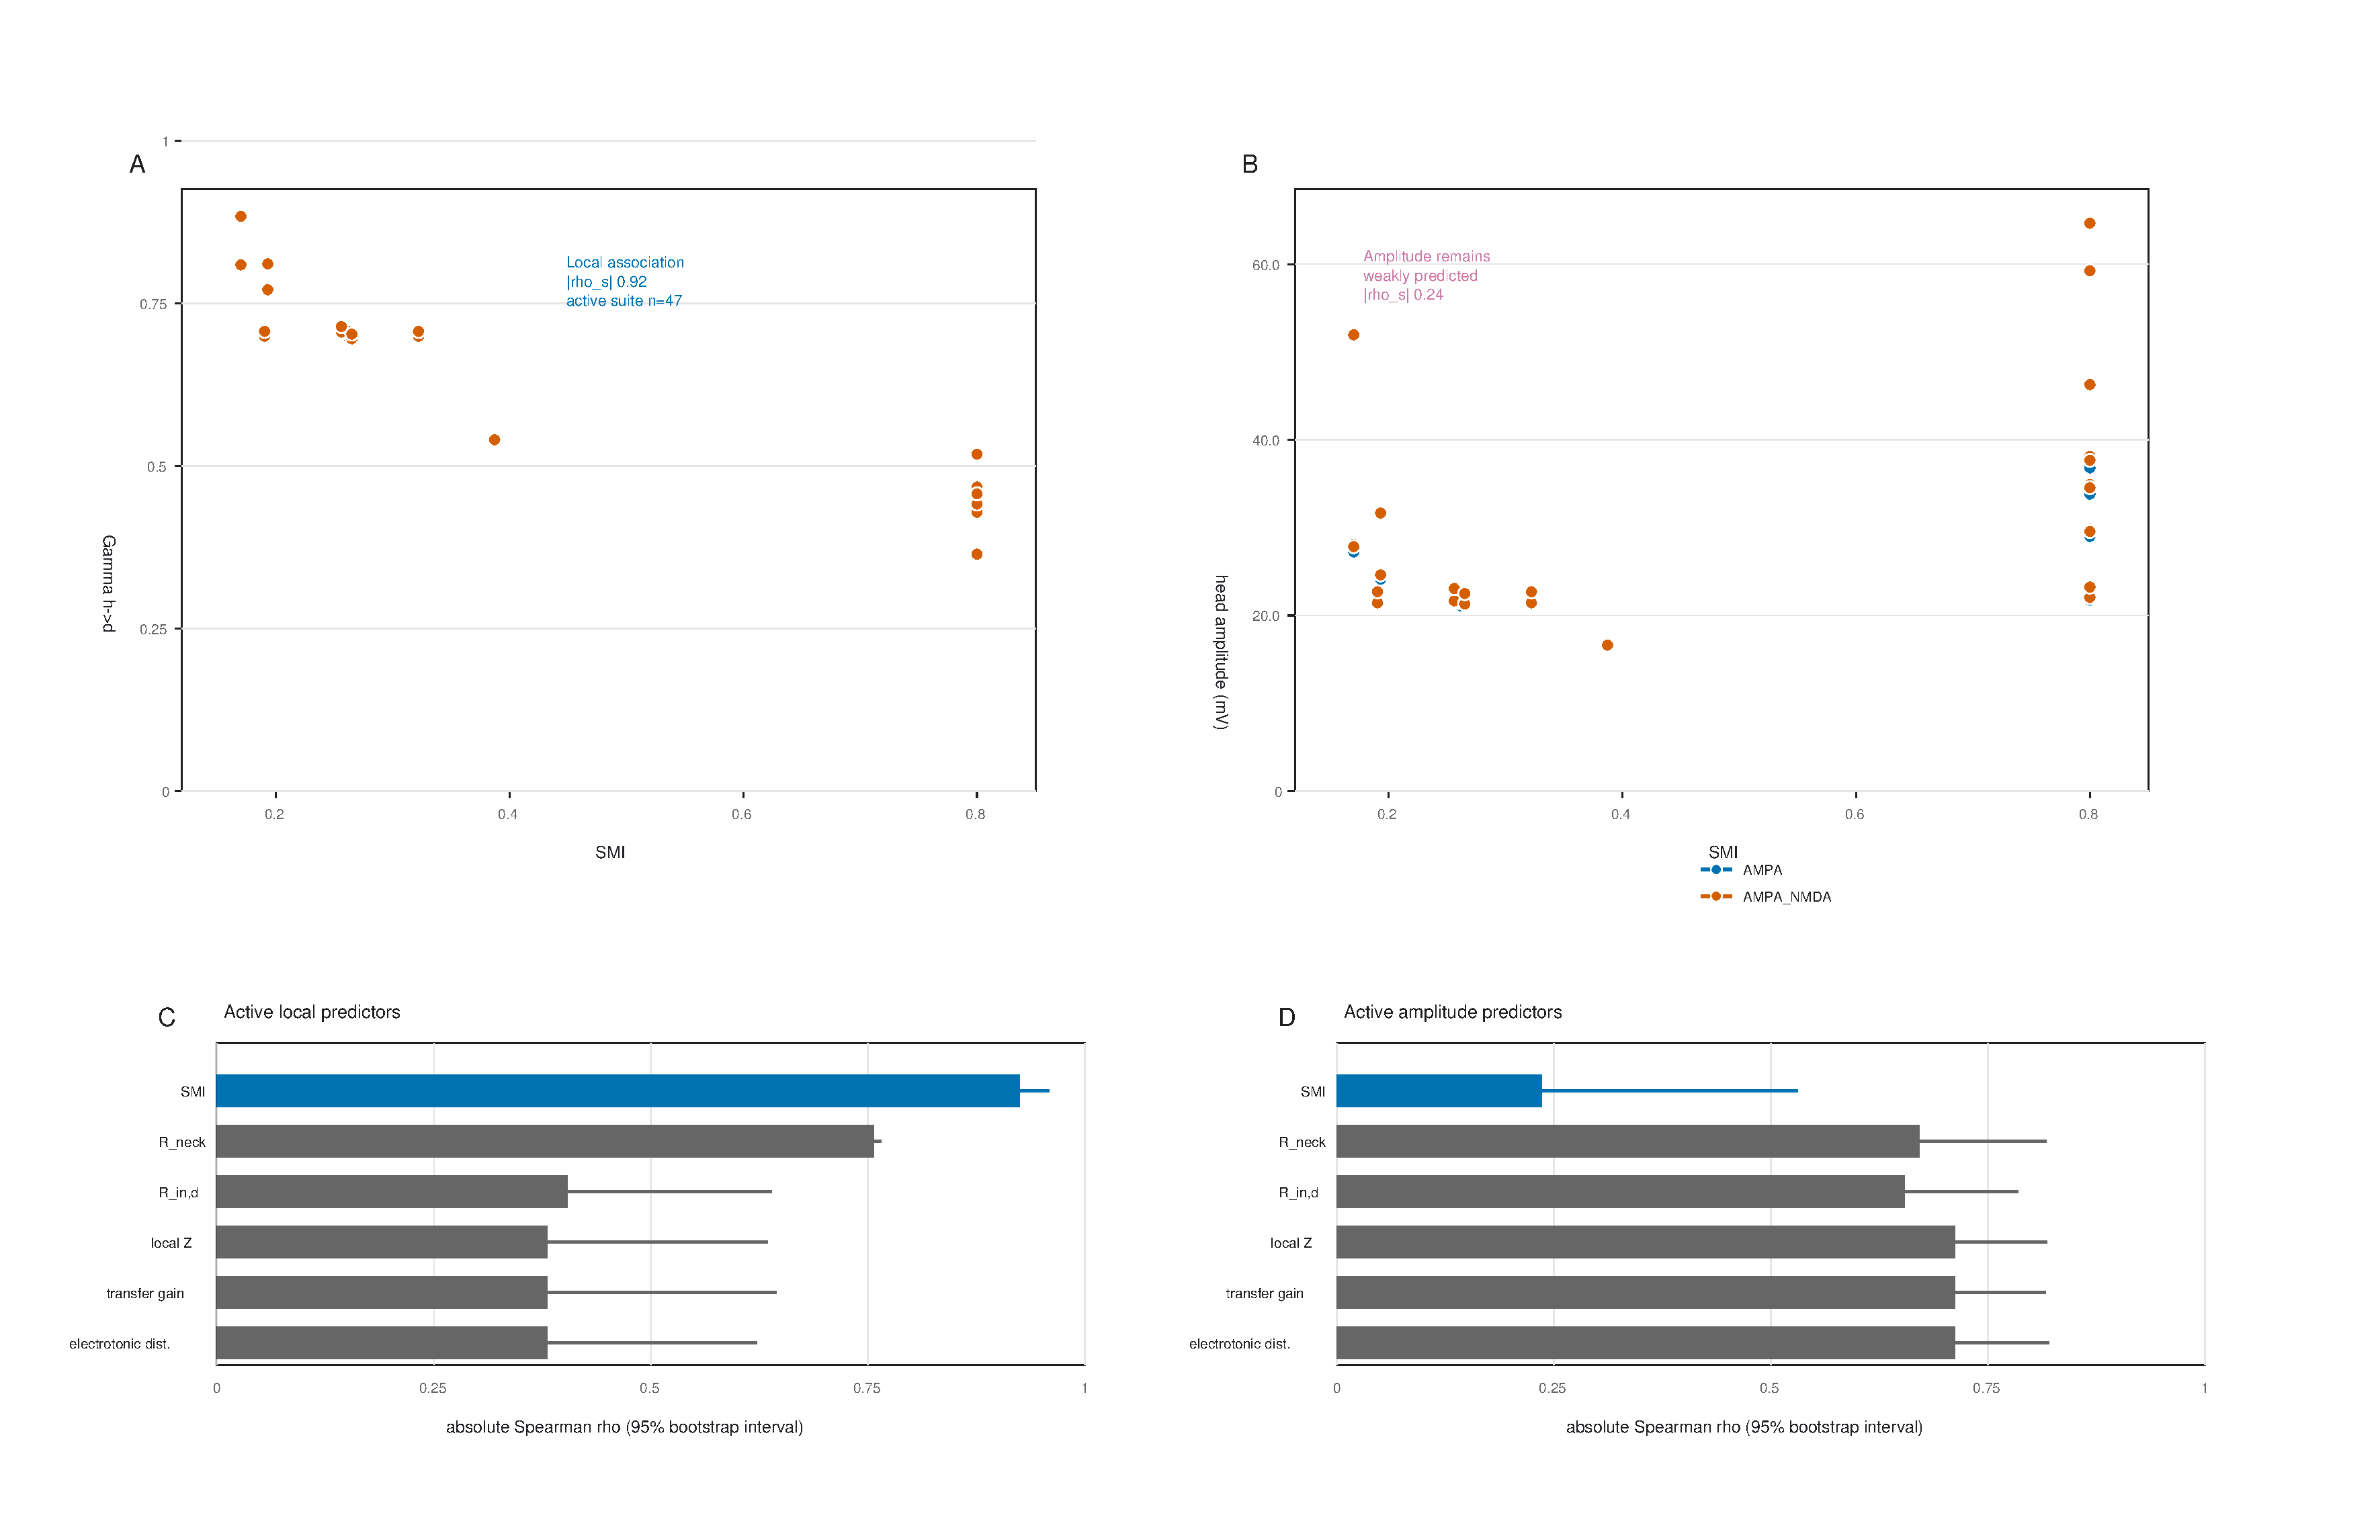
\includegraphics[width=\textwidth,keepaspectratio]{figures_publication/Fig6_active_domain.pdf}
\caption{\textbf{Active and NMDA stress-test boundaries.} Active and NMDA-enabled protocols retain local ratio ordering in designed cases but increase nonequivalence for amplitude and other response targets. These rows are generic stress tests rather than cell-type-calibrated active reconstructions.}
\label{fig:active}
\end{figure}

\subsection{Deterministic uncertainty stabilizes sampled low/intermediate behavior but not high-SMI claims}

Progressive uncertainty analysis resolved the small-sample instability seen in the original 48-versus-96 comparison. By N=768, final SMI median convergence passed: the 384-to-768 relative change was 0.012, below the predefined 0.10 threshold. The maximum final median relative change across tracked outputs was 0.029. Exact top-predictor ranking remained less stable than descriptor-family interpretation.

The N=768 ensemble does not support high-SMI uncertainty claims. It contained 757 low-SMI rows, 11 intermediate-SMI rows, and zero high-SMI rows. High-isolation conclusions therefore rest on baseline reference and designed challenge rows, not on the deterministic uncertainty ensemble.

Radius-only uncertainty produced 184 class flips out of 768 sampled parameter combinations, a design fraction of 24.0\%. Low-class combinations flipped in 22.9\% of cases, all 11 intermediate combinations flipped, and no high-SMI combinations were present. Because $\Rneck$ scales as $1/r_n^2$, continuous ratio values with explicit radius uncertainty are safer than treating low, intermediate, and high labels as sharply separated biological states.

\begin{figure}[!htbp]
\centering
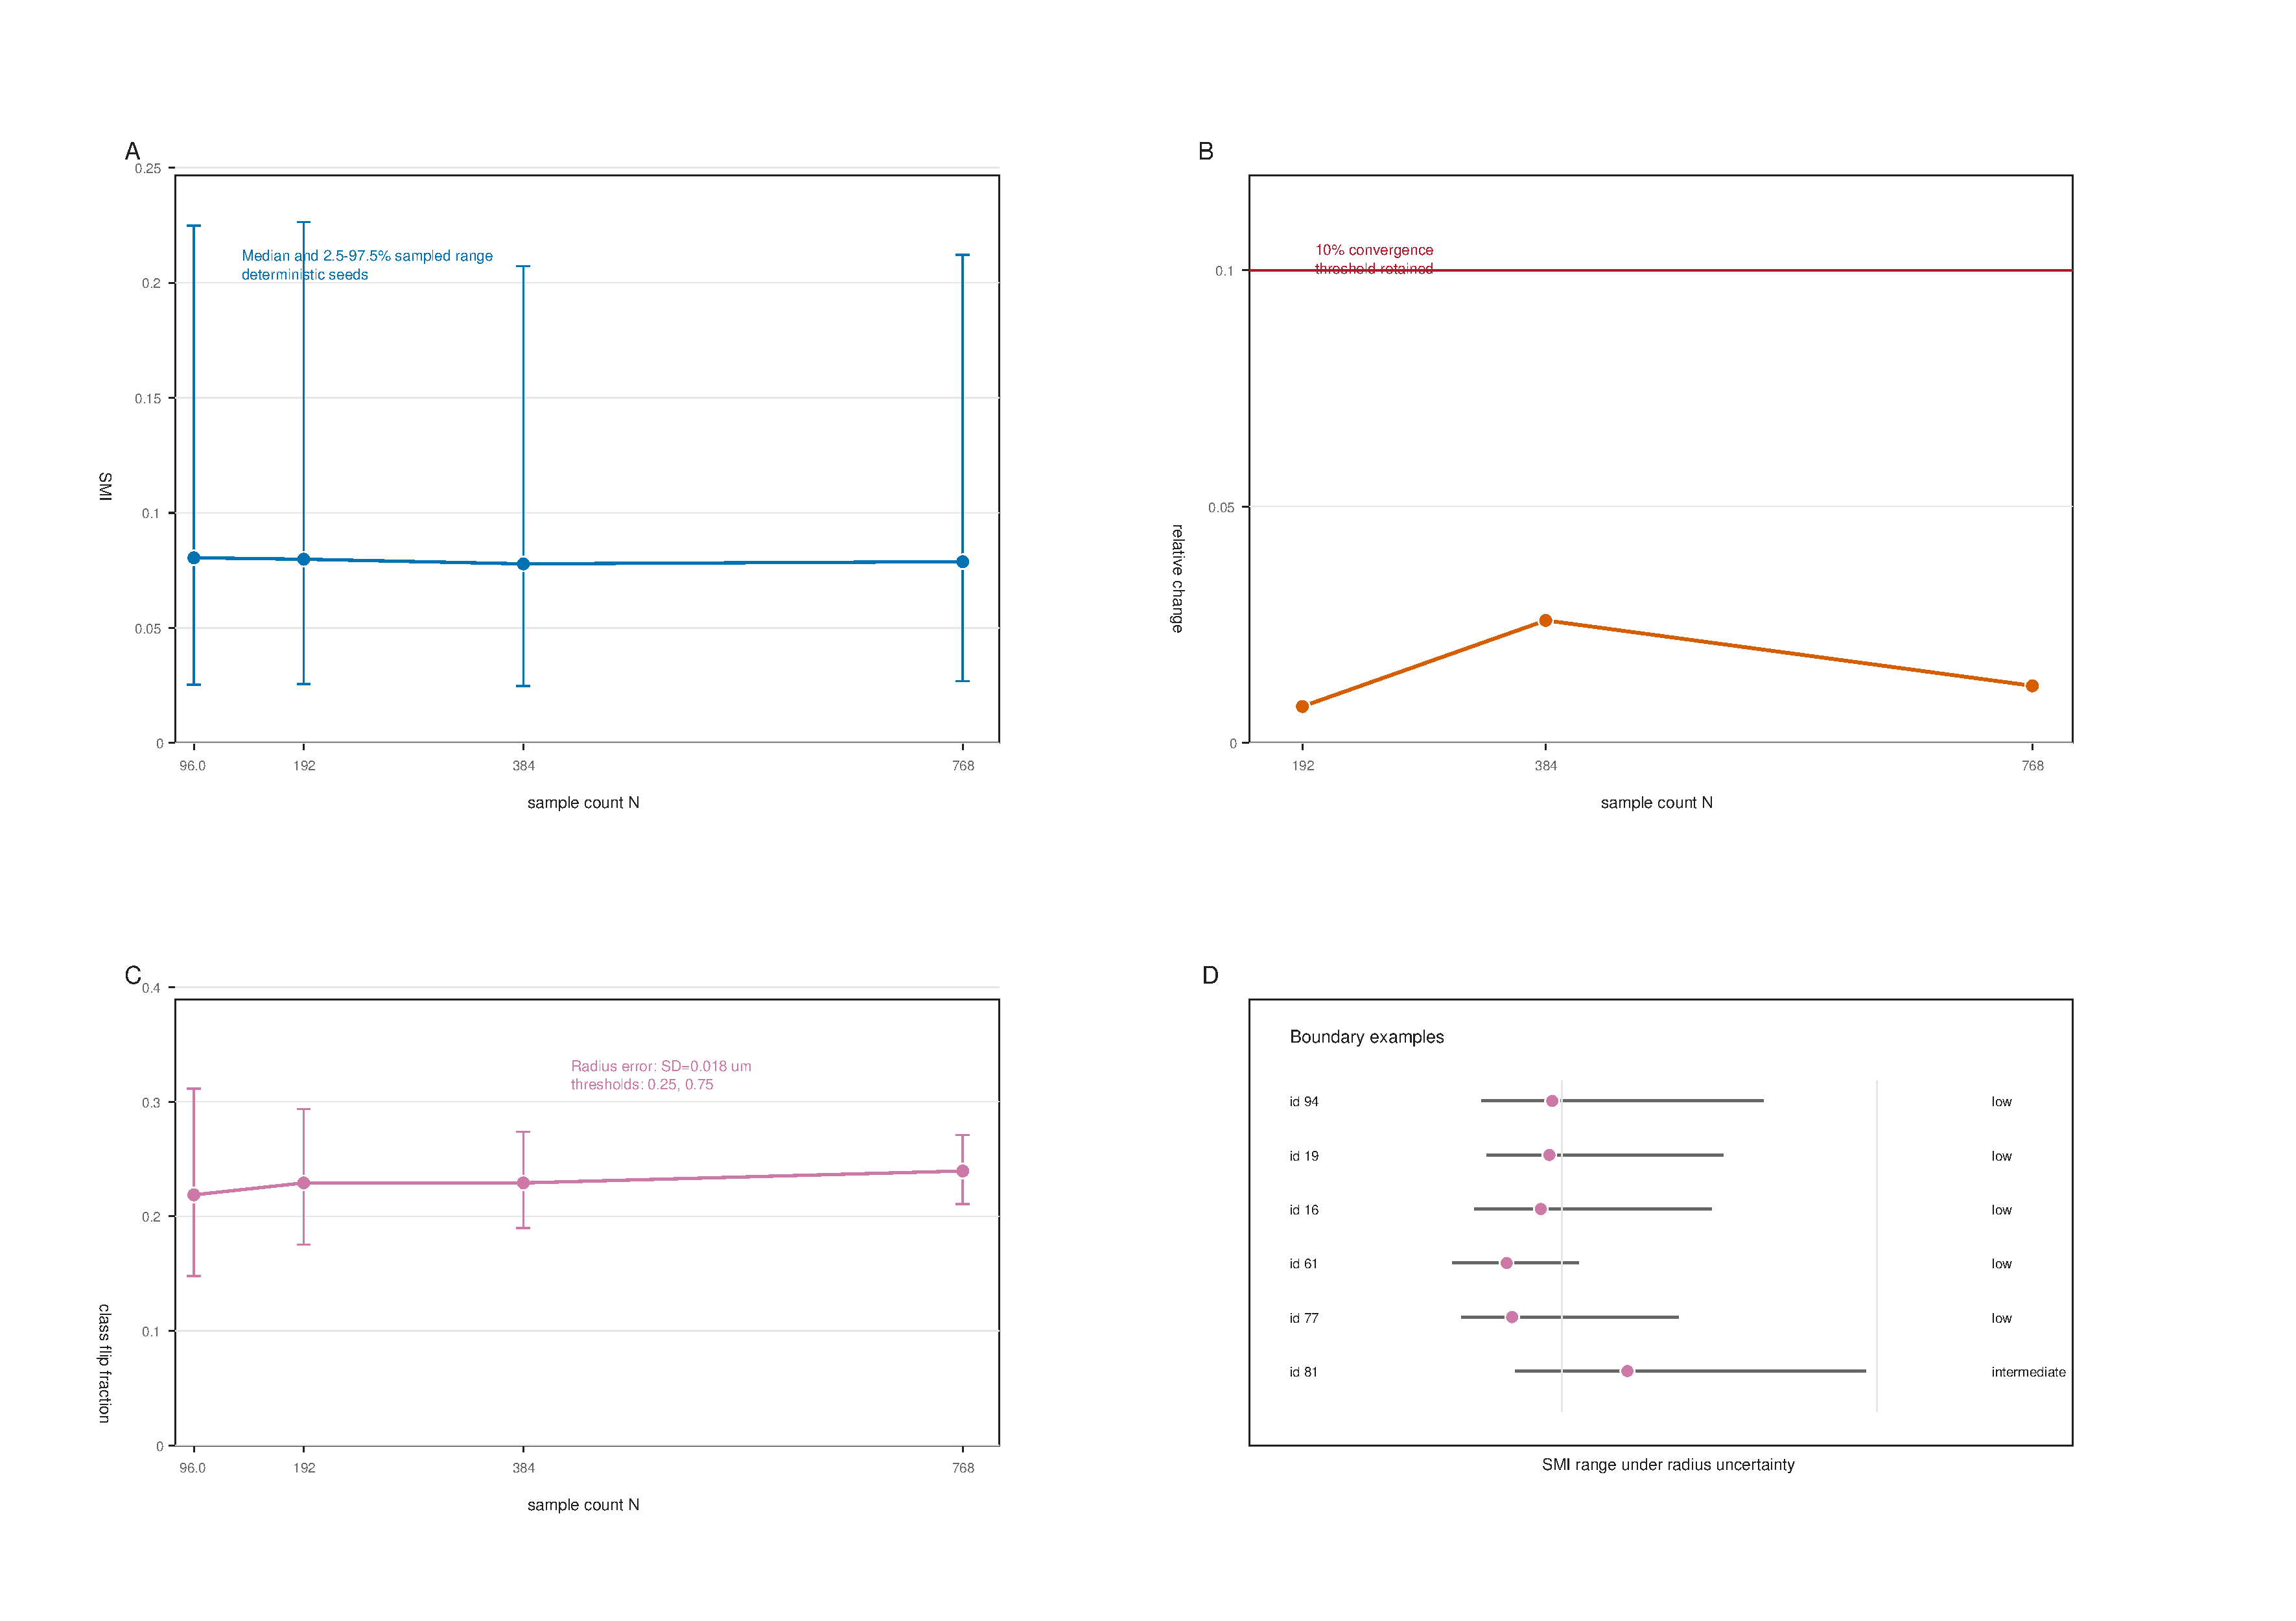
\includegraphics[width=\textwidth,keepaspectratio]{figures_publication/Fig7_uncertainty_radius.pdf}
\caption{\textbf{Deterministic uncertainty and radius sensitivity.} Progressive sampling stabilized continuous low/intermediate SMI summaries by N=768, while radius-error propagation exposed threshold-class fragility. Fractions are design fractions over sampled parameter combinations, not biological rates.}
\label{fig:uncertainty}
\end{figure}

\subsection{Independent benchmarks support computational credibility within scope}

Phase 4 addressed computational credibility beyond internal scheme agreement. An independently written direct-matrix implementation of the same passive three-compartment baseline reproduced existing SPINE baseline traces to numerical roundoff: the maximum all-trace absolute voltage difference was $1.25\times10^{-13}$ mV, the maximum head-amplitude difference was $1.42\times10^{-14}$ mV, and the maximum $\Ghd$ difference was $7.55\times10^{-15}$. DC analytic checks reproduced the two-node spine-omitted $\Rin$ value of 144.486692 M$\Omega$ to roundoff and confirmed the divider limits.

Backward Euler versus Crank-Nicolson peak differences were small in the baseline reference cases: maximum peak differences were 0.00203 mV for $\Ah$, 0.000534 mV for $A_d$, 0.000189 mV for $A_s$, and 0.000500 for $\Ghd$. These are internal numerical self-consistency checks. NEURON was unavailable in the execution environment, so no NEURON cross-check is claimed.

Earlier reviewer-access packages established manifest and checksum workflows. The finalization package supersedes those approval-gated drafts with a public release at \url{https://github.com/blakepi/spine-divider-residuals} and archival DOI \url{https://doi.org/10.5281/zenodo.20672333}.

\begin{table}[!htbp]
\centering
\caption{\textbf{Baseline reference passive parameters.} Values are taken from the manuscript-faithful baseline configuration and the three pre-specified reference neck geometries.}
\label{tab:parameters}
\resizebox{\textwidth}{!}{%
\begin{tabular}{lll}
\toprule
Parameter & Meaning & Value \\
\midrule
$E_L$ & leak reversal & -70 mV \\
$\Esyn$ & excitatory reversal & 0 mV \\
$c_m$ & specific capacitance & 0.01 pF $\mu$m$^{-2}$ \\
$\bar g_L$ & head specific leak & $3\times10^{-6}$ nS $\mu$m$^{-2}$ \\
$r_h$ & head radius & 0.35 $\mu$m \\
$C_d$, $C_s$ & dendrite and soma capacitance & 120 pF, 220 pF \\
$\gLd$, $\gLs$ & dendrite and soma leak & 2.5 nS, 7.0 nS \\
$\gDS$ & dendrite-soma coupling & 12.0 nS \\
$\rho_i$ & intracellular resistivity & 100 $\Omega$ cm \\
$g_{\max}$ & peak synaptic conductance & 1.4 nS \\
$\tau_r$, $\tau_d$ & rise and decay constants & 0.3 ms, 3.0 ms \\
$t_0$, $\Delta t$ & event time and time step & 20 ms, 0.01 ms \\
$T$ & metric window & 50 ms \\
$\Rin$ & spine-omitted dendrite-soma input resistance & 144.487 M$\Omega$ \\
low neck & $L_n$, $r_n$, $\Rneck$ & 0.25 $\mu$m, 0.25 $\mu$m, 1.273 M$\Omega$ \\
intermediate neck & $L_n$, $r_n$, $\Rneck$ & 0.75 $\mu$m, 0.12 $\mu$m, 16.579 M$\Omega$ \\
high neck & $L_n$, $r_n$, $\Rneck$ & 1.50 $\mu$m, 0.05 $\mu$m, 190.986 M$\Omega$ \\
\bottomrule
\end{tabular}}
\end{table}

